\usepackage{graphicx}
\usepackage{amsmath}
\usepackage{tikz}
\usepackage{hyperref}

\title{The World of Dungeons and Dragons}
\author{Your Name}
\date{\today}

\begin{document}
    \maketitle

    \tableofcontents
    \newpage


    \chapter{Introduction}\label{ch:introduction}
    Dungeons and Dragons (D\&D) is a popular tabletop role-playing game that has captivated the hearts of millions of players worldwide. In this paper, we will explore the fascinating world of D\&D, its history, gameplay, and cultural impact.


    \section{History of D\&D}\label{sec:history-of-d&d}
    The history of Dungeons and Dragons dates back to the 1970s when it was first created by Gary Gygax and Dave Arneson. It has since evolved through various editions and has become an iconic part of the gaming world.


    \chapter{Gameplay}\label{ch:gameplay}
    D\&D is known for its intricate gameplay mechanics. Players create characters, embark on adventures, and engage in collaborative storytelling.


    \section{Character Creation}\label{sec:character-creation}
    Creating a D\&D character involves selecting a race, class, and background. Players also determine their character's abilities, skills, and personality traits.


    \section{Adventures and Campaigns}\label{sec:adventures-and-campaigns}
    D\&D adventures are set in fantastical worlds filled with monsters, magic, and mysteries. Players participate in campaigns, guided by a Dungeon Master (DM), who acts as the storyteller and referee.


    \chapter{Monsters and Magic}\label{ch:monsters-and-magic}
    D\&D features a wide range of creatures and spells, adding depth and excitement to the game.


    \section{Notable Monsters}\label{sec:notable-monsters}
    From dragons to goblins, D\&D boasts a vast array of iconic monsters that challenge players throughout their adventures.

    \begin{figure}
        \centering
        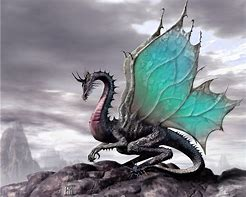
\includegraphics[width=0.6\textwidth]{dragon}
        \caption{An illustration of a fearsome dragon.}\label{fig:figure}
    \end{figure}


    \section{Magical Spells}\label{sec:magical-spells}
    Magic is an essential part of D\&D. Players can cast spells to heal, damage, or manipulate the world around them.

    \begin{equation}
        \label{eq:fireball}
        \text{Fireball Damage} = 8d6
    \end{equation}


    \chapter{Creating Game Maps}\label{ch:creating-game-maps}
    D\&D often requires intricate game maps for battles and exploration. To create these maps, the Tikz package in LaTeX can be a valuable tool.

    \begin{tikzpicture}
        \draw (0,0) -- (4,0) -- (4,4) -- (0,4) -- cycle;
        \node at (2,2) {Dungeon Map};
    \end{tikzpicture}


    \chapter{Tables}\label{ch:tables}
    Tables can be used to display information such as character stats, spell lists, or treasure hoards.

    \begin{table}[h]
        \centering
        \begin{tabular}{|c|c|c|}
            \hline
            Level & Hit Points & Armor Class \\
            \hline
            1     & 10         & 15          \\
            2     & 25         & 18          \\
            3     & 35         & 20          \\
            \hline
        \end{tabular}
        \caption{Character progression table.}\label{tab:table}
    \end{table}


    \chapter{Bibliography}\label{ch:bibliography}
    For more in-depth information on Dungeons and Dragons, consult the following references:

    \begin{enumerate}
        \item Gygax, Gary. \textit{Dungeons & Dragons Player's Handbook}. TSR, 1978.
        \item Cook, David "Zeb" et al. \textit{Player's Handbook (3.5e)}. Wizards of the Coast, 2003.
    \end{enumerate}

\end{document}
